%%%%%%%%%%%%%%%%%%%%%%%%%%%%%%%%%%%%%%%%%
% Thin Sectioned Essay
% LaTeX Template
% Version 1.0 (3/8/13)
%
% This template has been downloaded from:
% http://www.LaTeXTemplates.com
%
% Original Author:
% Nicolas Diaz (nsdiaz@uc.cl) with extensive modifications by:
% Vel (vel@latextemplates.com)
%
% License:
% CC BY-NC-SA 3.0 (http://creativecommons.org/licenses/by-nc-sa/3.0/)
%
%%%%%%%%%%%%%%%%%%%%%%%%%%%%%%%%%%%%%%%%%

%----------------------------------------------------------------------------------------
%	PACKAGES AND OTHER DOCUMENT CONFIGURATIONS
%----------------------------------------------------------------------------------------

\documentclass[a4paper, 11pt]{article} % Font size (can be 10pt, 11pt or 12pt) and paper size (remove a4paper for US letter paper)

\usepackage[protrusion=true,expansion=true]{microtype} % Better typography
\usepackage{graphicx} % Required for including pictures
\usepackage{wrapfig} % Allows in-line images
\usepackage{amsmath}
\usepackage{amsbsy}
\usepackage{amsthm}
\usepackage[space]{grffile}
\usepackage{color}
\usepackage{mathpazo} % Use the Palatino font
\usepackage[T1]{fontenc} % Required for accented characters
\linespread{1.05} % Change line spacing here, Palatino benefits from a slight increase by default
\newcommand{\LL}{\mathcal{L}}
\newcommand{\q}{\tilde{q}}
\newcommand{\x}{\tilde{x}}

%\makeatletter
%\renewcommand\@biblabel[1]{\textbf{#1.}} % Change the square brackets for each bibliography item from '[1]' to '1.'
%\renewcommand{\@listI}{sep=0pt} % Reduce the space between items in the itemize and enumerate environments and the bibliography
%
%\renewcommand{\maketitle}{ % Customize the title - do not edit title and author name here, see the TITLE block below
%\begin{flushright} % Right align
%{\LARGE\@title} % Increase the font size of the title
%
%\vspace{50pt} % Some vertical space between the title and author name
%
%{\large\@author} % Author name
%\\\@date % Date
%
%\vspace{40pt} % Some vertical space between the author block and abstract
%\end{flushright}
%}

%----------------------------------------------------------------------------------------
%	TITLE
%----------------------------------------------------------------------------------------

%\title{\textbf{Unnecessarily Long Essay Title}\\ % Title
%Focused and Deliciously Witty Subtitle} % Subtitle
%
%\author{\textsc{Ford Prefect} % Author
%\\{\textit{Interstellar University}}} % Institution
%
%\date{\today} % Date

%----------------------------------------------------------------------------------------
\graphicspath{{/Users/zhaolong/Google Drive/Kumar/StorageNG/LongCode/Meeting/}}

\begin{document}

%\maketitle % Print the title section

%----------------------------------------------------------------------------------------
%	ABSTRACT AND KEYWORDS
%----------------------------------------------------------------------------------------

%\renewcommand{\abstractname}{Summary} % Uncomment to change the name of the abstract to something else

%\begin{abstract}
%
%\end{abstract}
%
%\hspace*{3,6mm}\textit{Keywords:} lorem , ipsum , dolor , sit amet , lectus % Keywords
%
%\vspace{30pt} % Some vertical space between the abstract and first section

%----------------------------------------------------------------------------------------
%	ESSAY BODY
%----------------------------------------------------------------------------------------

%\section*{Introduction}

\begin{enumerate}

 \item Why last time's curve is so smooth?\\

Since the discount rate $\beta = 0.3$ which is huge, it is intuitive to think that only the first several transactions make a difference. This intuition is verified by the following five figures.\\



\begin{figure}
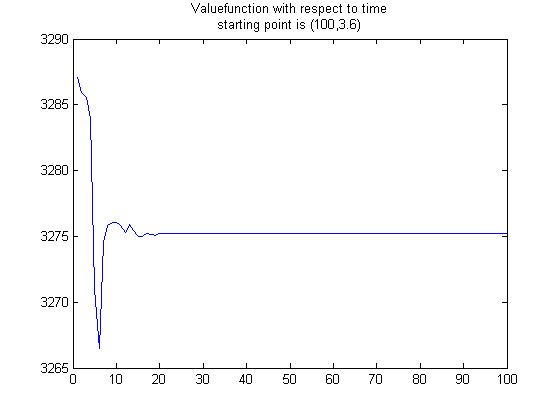
\includegraphics[scale = 0.65]{originalValueTimeQmaxXmax.jpg}
\end{figure}


\begin{figure}
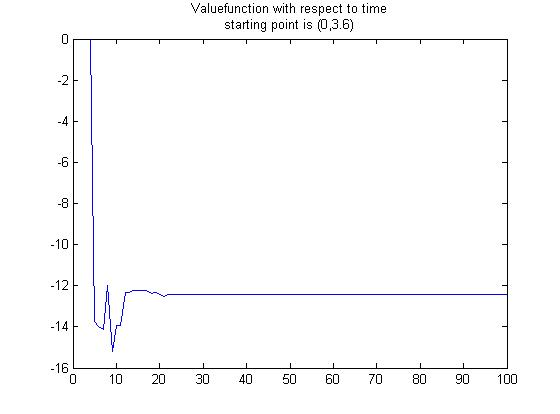
\includegraphics[scale = 0.65]{originalValueTimeQminXmax.jpg}
\end{figure}

\begin{figure}
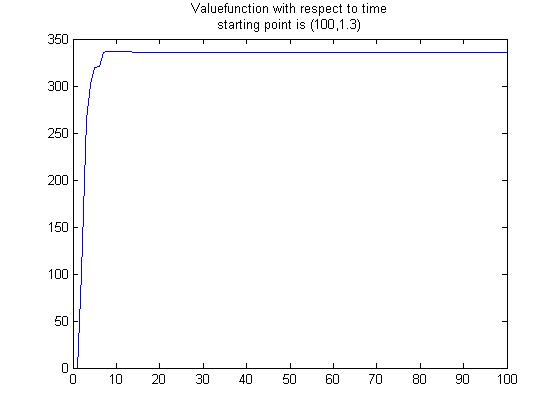
\includegraphics[scale = 0.65]{originalValueTimeQmaxXmin.jpg}
\end{figure}


\begin{figure}
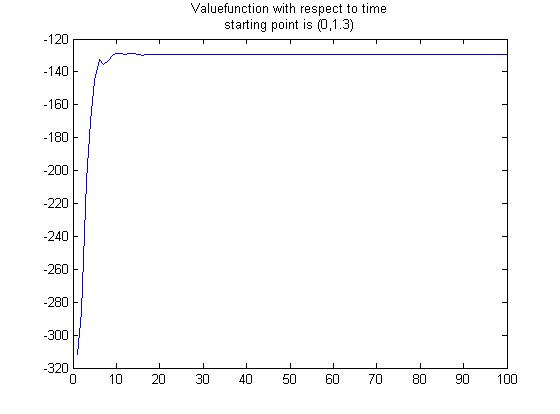
\includegraphics[scale = 0.65]{originalValueTimeQminXmin.jpg}
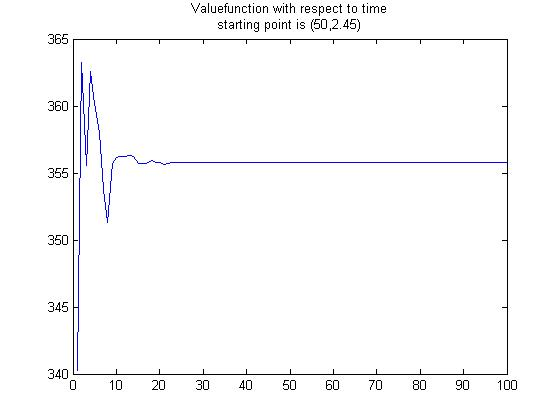
\includegraphics[scale = 0.65]{originalValueTimeQmidXmid.jpg}
\end{figure}

%\begin{figure}
%
%\end{figure}

%\starting point is four vertexes and one point in the middle.

\newpage

For most points that belong to selling region, the initial selling profit (selling at time $0$) is nearly the same as the value function itself.\\

\begin{figure}[p]
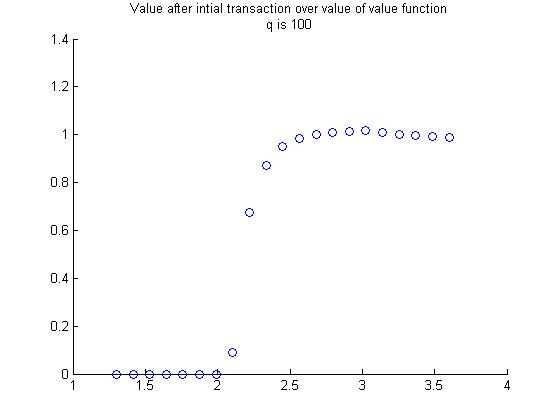
\includegraphics[scale = 0.65]{originalInitialRatioQmax.jpg}
\end{figure}

\begin{figure}[p]
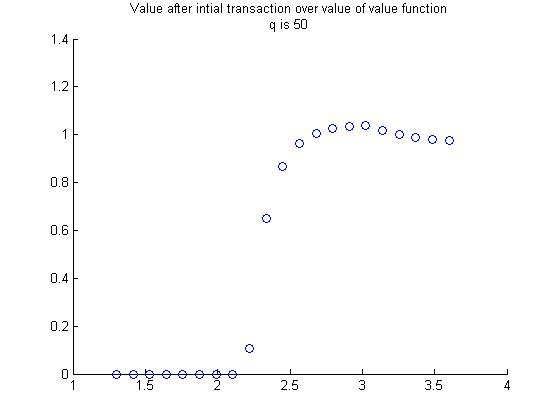
\includegraphics[scale = 0.65]{originalInitialRatioQmid.jpg}
\end{figure}
%give two ratio plots one for q = Qmax, one for q = (Qmin+Qmax)/2


\newpage
The reason why the above is true is that the first transaction is the only transaction for a relatively long time\footnote{By saying relative long, I mean that the discount rate at the end of this time period is very small}. Below is a path from starting point$(Q_{max},X_{max})$.\\

\begin{figure}
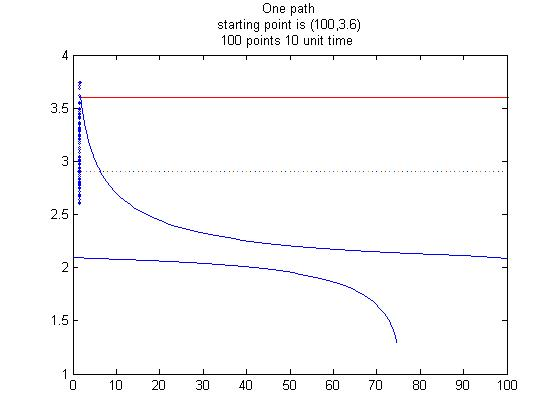
\includegraphics[scale = 0.65]{originalOnePathQmaxXmax.jpg}
\end{figure}

%give a one path plot for starting point Qmax Xmax

\newpage 
The plot of boundary is as following. It is worth to notice that the selling boundary is below the mean reverting level $\alpha$ and buying boundary is a little bit far away from $\alpha$. This means that the top left corner is like a dead end of the whole process. This can also be seen from the fact that the value of value function at that region is close to $0$. I would like to introduce the main idea about the process by by an example. \\

\begin{figure}
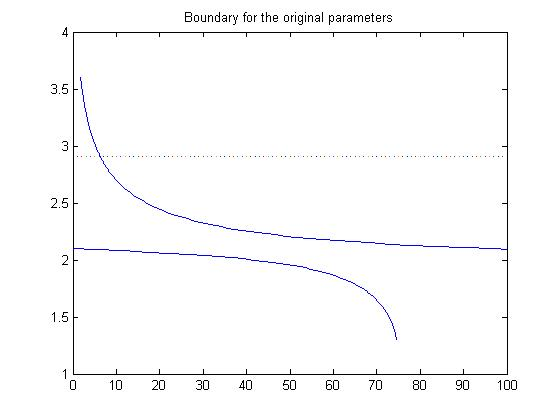
\includegraphics[scale = 0.65]{originalBoundary.jpg}
\end{figure}

\newpage
Starting from $(0,1.3)$ (the left bottom point), we will buy about $75$ products. Since the selling boundary is below $\alpha$, we will sell part of it quite quickly like $1$ unit time. After this, the price is still below the $\alpha$,  therefore it will increase which means that we will sell it again in a short time. This will continue until we are above $\alpha$ with little storage. Then the price will go up and down near $\alpha$, however, since the buying boundary is kind of far away, we won't buy anything in a relative short time, so the main value is from buying a huge a mount and sell it several times until the price is above $\alpha$. Even the price may decrease again and we may buy again during the process, but as said before, we will sell it quite quickly which doesn't change the main idea.\\

\begin{figure}
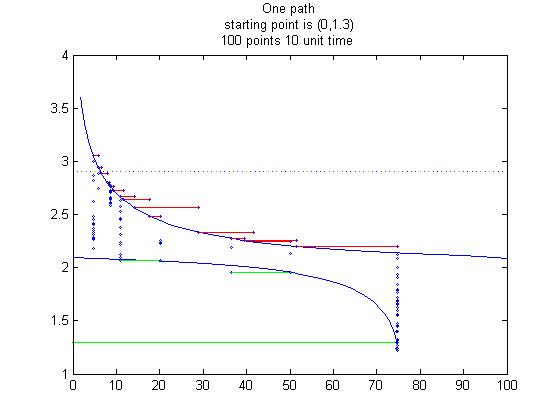
\includegraphics[scale = 0.65]{originalOnePathQminXmin.jpg}
\end{figure}


%insert the original_Qmin_Xmin
\newpage
Noticing that the selling transaction cost is increasing with respect to the volume, when we sell the product at a low price, the transaction cost we pay is also low. What's more,  even we may buy the product at a low price again during the process, because of the transaction cost, we may not be able to sell it for a profit. For example, in the above figure, we buy $15$ units at $x = 1.9$ and sell it again at $x =2.25$. Even though the price difference is $\exp(2.25) -\exp(1.9) = 2.8$, however the transaction cost per unit is about $2$ ($1$ for buying and $1$ for selling). Adding the discount factor, we can barely make any profit by buying low and selling high. \\


All in all, the main part of value function will come from \\

\begin{enumerate}

\item Left top. We will remain at the holding region.(See the figure on the page)

\begin{figure}
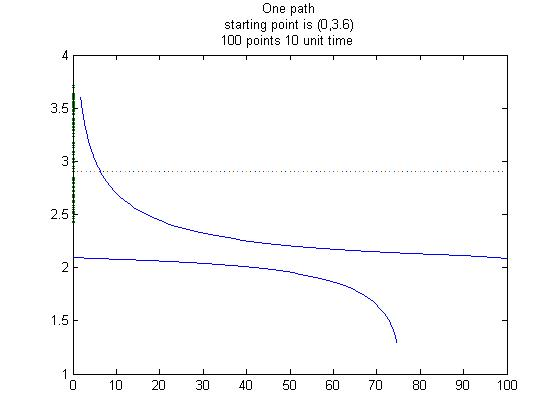
\includegraphics[scale = 0.65]{originalOnePathQminXmax.jpg}
\end{figure}

\newpage
\item Right top. Initial transaction is the main thing, after it we bare do anything.

\item Left bottom. We will buy a lot of products at time $0$, and all the things left is to sell it.

\item Right bottom. Wait the price increase and we will sell what we have at the beginning. (See the figure on the page)

\begin{figure}
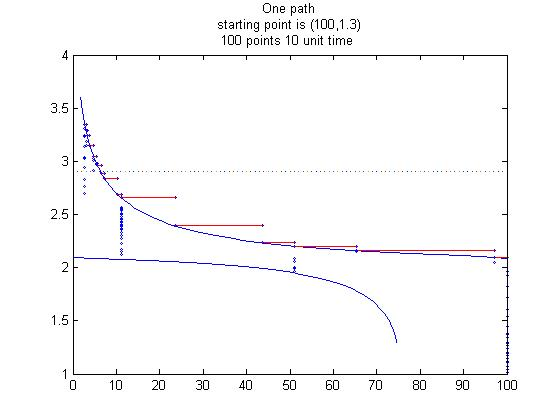
\includegraphics[scale = 0.65]{originalOnePathQmaxXmin.jpg}
\end{figure}

\newpage
\item Middle. Buy and sell a lot of times and eventually will end at the left top (Dead end).(See the figure on the page)

\begin{figure}
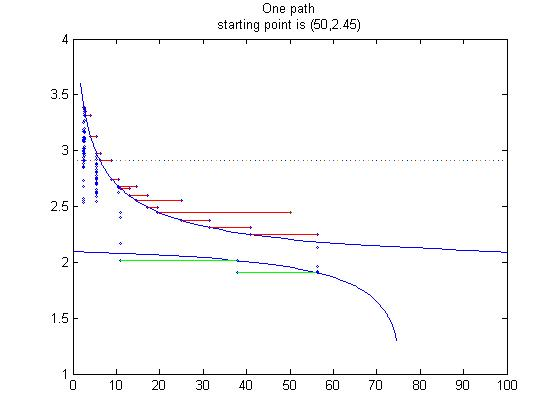
\includegraphics[scale = 0.65]{originalOnePathQmidXmid.jpg}
\end{figure}

\end{enumerate}

\newpage
The standard deviations are extremely small for the points at the right top and left top, because we barely do anything there.\\

%give two plots one for q = Qmax, one for q = 0. N =10000

\begin{figure}
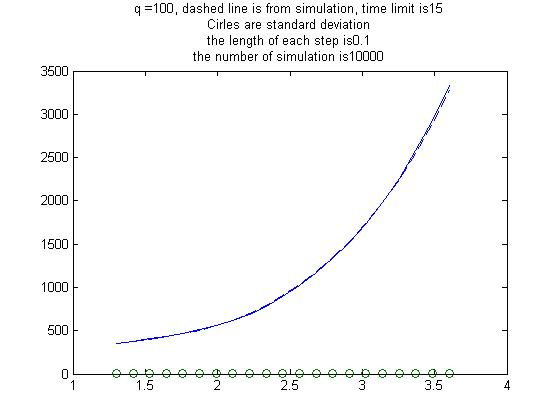
\includegraphics[scale = 0.65]{originalTwoValuesAndSD.jpg}
\end{figure}


The strategy we used here is quite conservative because we won't buy unless at a low price and we will sell if it increase a little bit. The value function for this strategy is very likely to be positive and this is the reason why I choose these unrealistic parameters.\\


   


\item However, above case is not that interesting due to the following reasons.\\

\begin{enumerate}

\item The parameters are unrealistic.

\item Selling is dominating buying.

\item It will go to a dead end which makes it less random.

\end{enumerate}

Therefore, I choose the new parameters (shown at the last page) and boundary which is shown below. First, let us see the boundary of the problem.\\

%The boundary with respect to the new parameters.
\begin{figure}
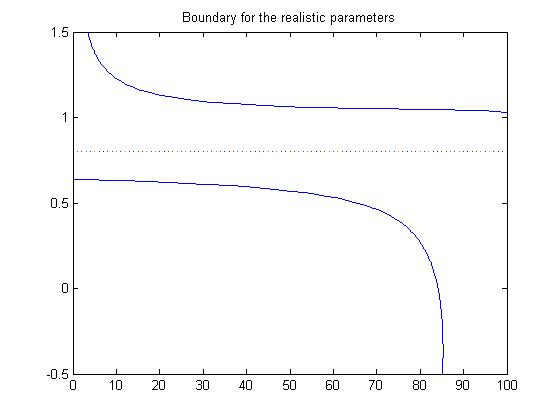
\includegraphics[scale = 0.65]{Stathis1Boundary.jpg}
\end{figure}


Unlike before, the selling boundary is not under mean reverting level $\alpha$ and the boundaries are relatively close to $\alpha$. We may expect that the total amount of transactions will be quite larger than previous case by which I mean the total amount we buy and sell quite larger than just $Qmax$ which is in the previous case.\\

%The plots of one path starting from Qmin Xmin, Qmid Xmid Qmax Xmax. And give the average number of buying and selling.
\begin{figure}
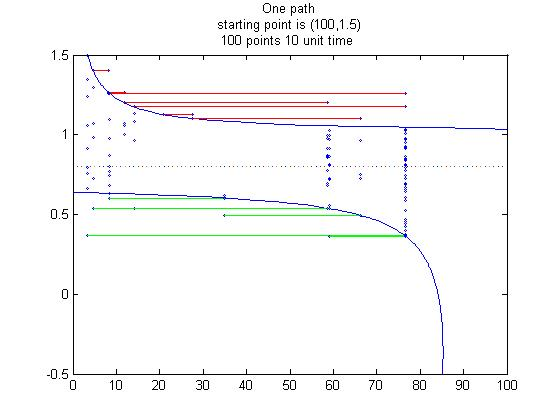
\includegraphics[scale = 0.65]{Stathis1OnePathQmaxXmax.jpg}
\end{figure}

\begin{figure}
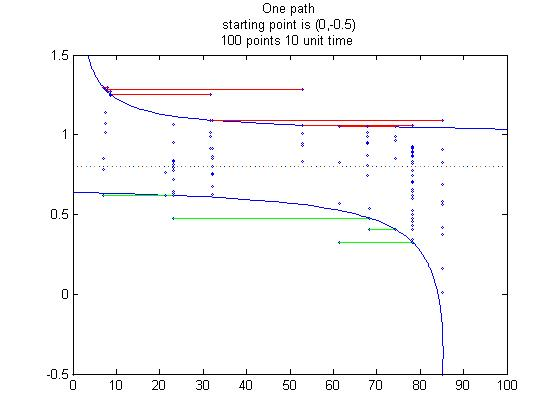
\includegraphics[scale = 0.65]{Stathis1OnePathQminXmin.jpg}
\end{figure}

\begin{figure}
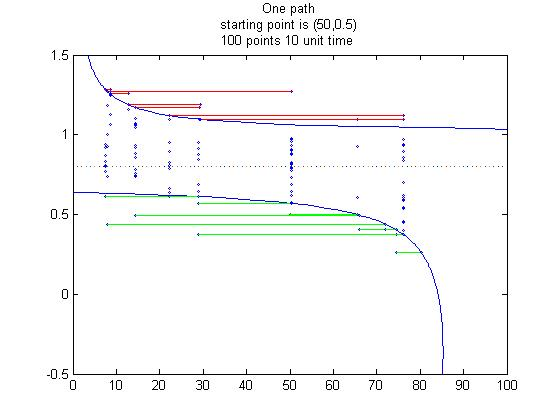
\includegraphics[scale = 0.65]{Stathis1OnePathQmidXmid.jpg}
\end{figure}

\newpage
Since the discount rate $\beta$ is low, the value function will be affected by the events happens long time after initial time.\\

%The plots of VTime starting from Qmax Xmin QmidXmid QminXmax(Because QmaxXmax and QminXmin will be transacted into QmaxXmin and QminXmax by the initial transaction

\begin{figure}
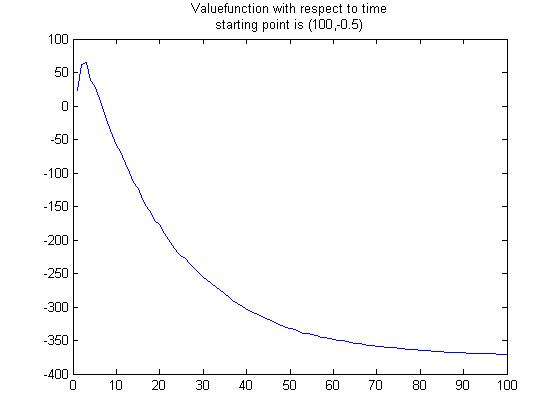
\includegraphics[scale = 0.65]{Stathis1ValueTimeQmaxXmin.jpg}
\end{figure}

\begin{figure}
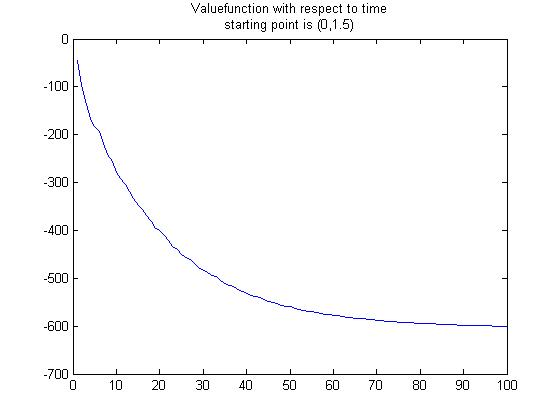
\includegraphics[scale = 0.65]{Stathis1ValueTimeQminXmax.jpg}
\end{figure}

\begin{figure}
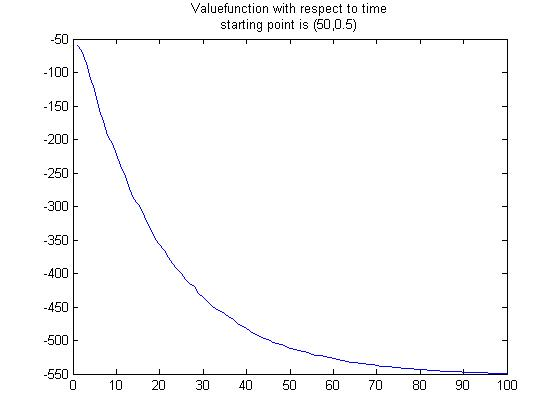
\includegraphics[scale = 0.65]{Stathis1ValueTimeQmidXmid.jpg}
\end{figure}



\newpage
However, the two methods give me the totally different values.\\

%The plots of valuePDE and value sim with tau = 0.1. With Qmax ( I should include the variance)

\begin{figure}
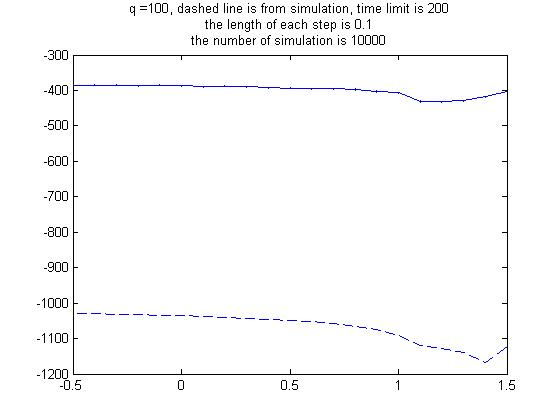
\includegraphics[scale = 0.65]{Stathis1TwoValuesAndSDQmaxDot1.jpg}
\end{figure}

\newpage
Even though they are totally different values, the trends of them are quite similar.\\

%The plotyy of valuePDE and value sim.

\begin{figure}
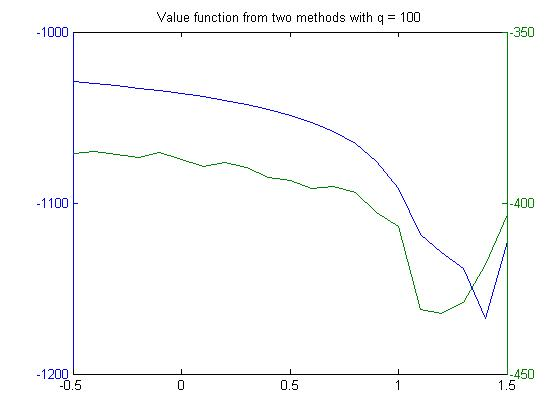
\includegraphics[scale = 0.65]{Stathis1TwoValuesQmaxYY.jpg}
\end{figure}
\newpage
What's more, when we apply the discrete PDE operator$A\times V- b$ to the value function obtained by simulation, we have the value is quite close to $0$ comparing with the scale of value function.\\

%The plotyy of the residual and valuePDE with Qmax
\begin{figure}
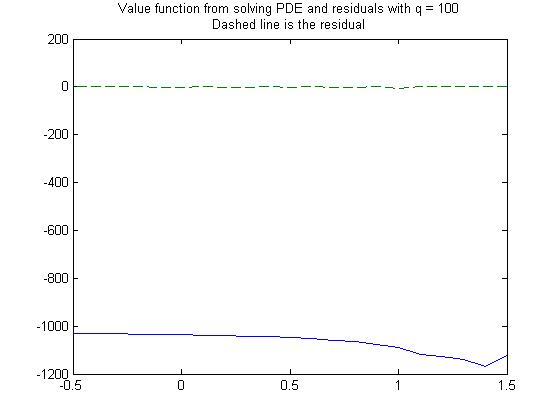
\includegraphics[scale = 0.65]{Stathis1ValuesAndResidualsQmax.jpg}
\end{figure}

\newpage
Which one is wrong? Value from solving PDE or value from simulation? Actually, at first I think that both of them can't be wrong because they matched when using another set of parameters. \\ 

If it is the value from PDE that is wrong, then adding discrete points must will help us decrease the gap. 
\begin{enumerate}

\item Increasing NumQ.

\item Increasing NumX.

\item Increasing NumX and NumQ together.

\end{enumerate}



However, we can't do this directly by changing NumX and NumQ directly in the code, because the way we choose the Xmax and Xmin. There are several rules needed to following in order to choose the Xmax and Xmin with given NumX and NumQ.\\

\begin{enumerate}
\item Only point (Xmax,Qmin) should be in the holding region while all other points (Xmax, q) should be in selling region, because the boundary condition for a top holding region is based on the fact that there should be no selling region above it ( by above I mean along X axis).

\item Similar things we need to consider when we choose Xmin. Because the boundary condition for a bottom holding region is based on the fact that there should be no buying region below the it, at Xmin, the boundary should have reached the largest q that it is able to achieve.

\item We still need to make sure that the points belong to holding region is enough to do the calculations. If we can't guarantee this, we need to choose a new pair of NumX NumQ.

\end{enumerate}

% The plot of NumX =20, NumQ = 20, 40,100
\begin{figure}
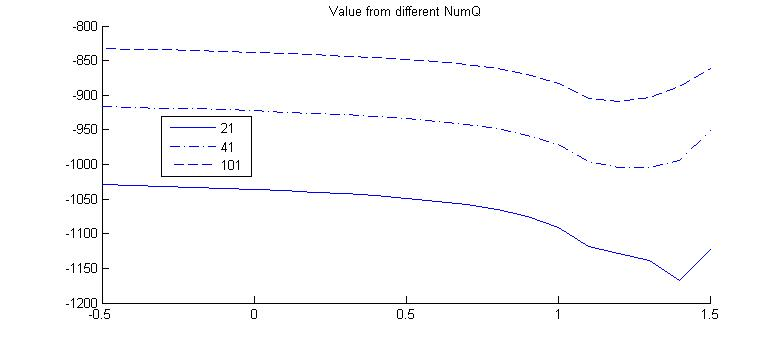
\includegraphics[scale = 0.5]{Stathis1ValueWithDiffNumQ.jpg}
\end{figure}

\begin{figure}
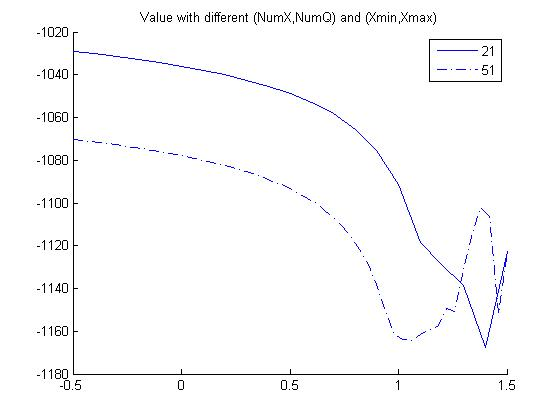
\includegraphics[scale = 0.65]{Stathis1ValueWithDiffNumQNumXXminXmax.jpg}
\end{figure}

\newpage
If it is the value from simulation that is wrong, then doing the following things should help us decrease the gap.\\

\begin{enumerate}

\item Increasing $T$. The plot of value changes with respect to time shows that it should not be a issue.

\item Increasing $N$. This will only decrease the standard deviation but not the level of the value.

\item $\tau$ the length of each time segment. It turns out to be the reason.

\begin{figure}
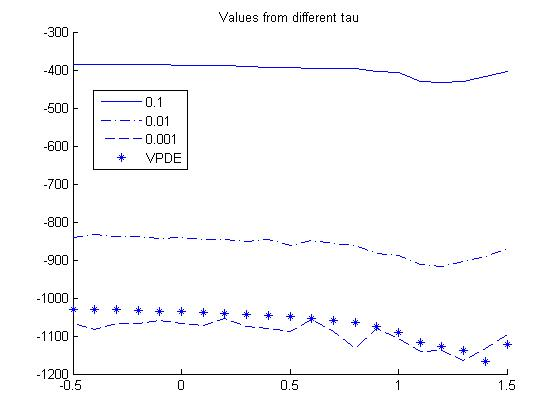
\includegraphics[scale = 0.65]{Stathis1ValueWithDifftau.jpg}
\end{figure}

($\tau = 0.1, N =10000$, $\tau = 0.01, N = 1000$, $\tau = 0.001, N =100$.)

\begin{figure}
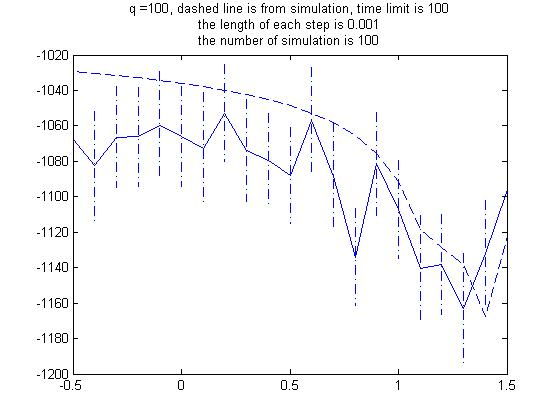
\includegraphics[scale = 0.65]{Stathis1TwoValuesAndSDQmaxDot001.jpg}
\end{figure}


% The plot of value with \tau = 0.1,0.01,0.001 with value from PDE as benchmark

\end{enumerate}

\newpage

Why it is the case? The initial transaction doesn't count nearly at all (because all the value is negative and initial transaction of selling is positive) and the value changes a lot with respect to time. Therefore, all that matter are the transaction along time. If we do it continuously, it should moving along the boundary. However, when $\tau$ is big, it will not move like this.\\

%The plot of one path for \tau = 0.1, \tau = 0.01, \tau = 0.001
\begin{figure}
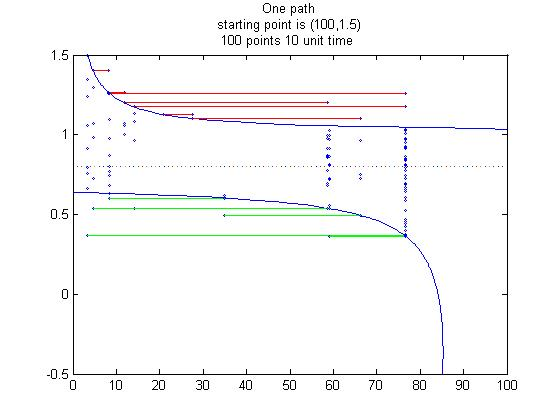
\includegraphics[scale = 0.65]{Stathis1OnePathQmaxXmax.jpg}
\end{figure}

\begin{figure}
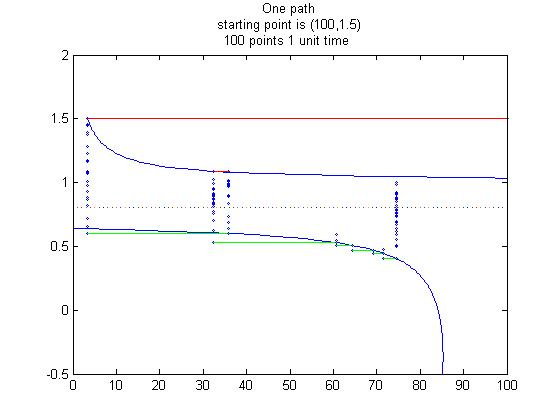
\includegraphics[scale = 0.65]{Stathis1OnePathQmaxXmaxDot01.jpg}
\end{figure}

\begin{figure}
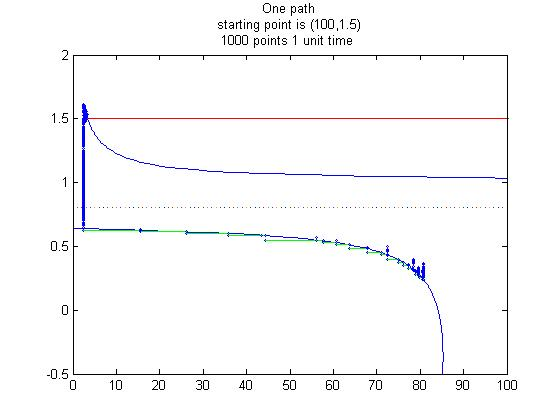
\includegraphics[scale = 0.65]{Stathis1OnePathQmaxXmaxDot001.jpg}
\end{figure}


\newpage

If it jumps into the buying region, it can buy with a lower price. If it jumps into the selling region, it can sell with a higher price. Therefore the value with large $\tau$ is bigger than the value with small $\tau$.\\

The reason why the value function is decreasing is because all the values using this strategy are all negative. The point with low price ($Q = 100$ for all), will start the first transaction later than those points with initial transaction. Which means the value is a ratio of a negative number which means that it is larger than the value at a high price. \\

From the plot of value PDE, we can see that the trend in the selling region is quite random.\\
% It is amazing that what I have said is true!!!
%I need to plot it with different NumX and NumQ but have the same points with in the smaller region.

\newpage

From the figure on this page, we know that it is the transaction cost that make the value negative.\\

\begin{figure}
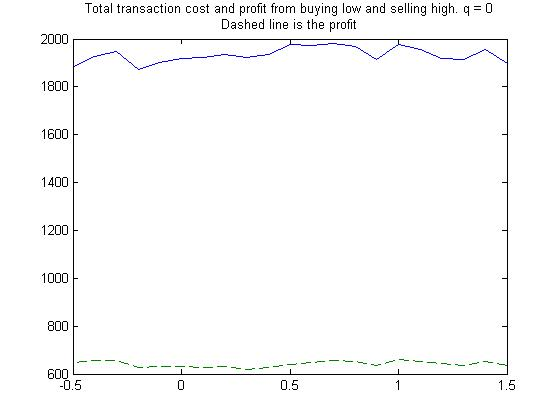
\includegraphics[scale = 0.65]{Stathis1TotalTranCosts.jpg}
\end{figure}


%the plot of boundary

%Give a picture to show that the boundary is far away and barely buy or sell. (Use the original plot instead of the new one. If I made a mistake, I admit it and do even harder the next time.)
%
% Point out that the buying curve is concave while the selling curve is convex which makes it impossible to transact after first transaction. 
%
% Give the average number of buying and selling. This number should be around $2$. Calculate the number of $\exp(-50*0.3)*10* \exp(4) = 1.6 \times 10^{-4}$.
%
% 
%
% However, the most important case should not be this case, therefore we should push the boundary down but make sure that the holding region is still big enough to be numerically precise in some sense.
%\end{enumerate}
%
% Nearby Boundary
%
%\begin{enumerate}
%
% Give the plot of the boundary.
%
% Give one path of the boundary. Starting from different initial point.
%
% Give the average number of buying and selling. Give a plot as well.
%
%
%
%\end{enumerate}
%
\end{enumerate}

%\newpage
%\section{Problems}
%
%When increase $NumX$ and $NumQ$, it is quite often that the results are quite different.
%
%\begin{enumerate}
%
%\item  Increasing NumX.
%\begin{enumerate}
%
%\item%The plot of NumX =20, NumX = 40,NumX =100 for original parameters
%\item%The plot of NumX =20, NumX = 40,NumX =100 for Stathis parameters
%
%\end{enumerate}
%
%\item Increasing NumQ.
%\begin{enumerate}
%\item%The plot of NumX =20, NumX = 40,NumX =100 for original parameters
%\item%The plot of NumX =20, NumX = 40,NumX =100 for Stathis parameters
%\end{enumerate}
%\end{enumerate}


\newpage
The value of unrealistic parameters are as following.

\begin{equation*}
\begin{split}
& \kappa = .301\\
& \sigma = .334\\
& \alpha =2.907\\
& \beta = 0.3 \quad \mbox{This is the discount rate for unit time of simulation}\\
& Xmin = 1.3\\
& Xmax = 3.6\\
&Qmin = 0\\
&Qmax = 100\\
& NumX = 21\\
&NumQ =21\\
&tau = 0.1 \quad \mbox{The length of each step in simulation}\\
&T = 100 \quad \mbox{The time limit of simulation}\\
\end{split}
\end{equation*}



The value of realistic parameters are as following.

\begin{equation*}
\begin{split}
& \kappa = 3.4\\
& \sigma = 0.59\\
& \alpha =0.802\\
& \beta = 0.05 \quad \mbox{This is the discount rate for unit time of simulation}\\
& Xmin = -0.5\\
& Xmax = 1.5\\
&Qmin = 0\\
&Qmax = 100\\
& NumX = 21\\
&NumQ =21\\
&tau = 0.1 \quad \mbox{The length of each step in simulation}\\
&T = 100 \quad \mbox{The time limit of simulation}\\
\end{split}
\end{equation*}

%[rgb]{1,0,0}
\end{document}